% !TEX TS-program = xelatex

% Inicializace tulthesis
\documentclass[FM,Proj]{tulthesis}
\usepackage{polyglossia}
\setdefaultlanguage{czech}
\usepackage{xevlna}

% Pro umisťování obrázků
%\usepackage{float}

% Pro seznam použité literatury
\usepackage[backend=biber, style=iso-numeric]{biblatex}
\addbibresource{zdroje.bib}

% Titulní strana
\TULtitle{Vývoj akční videohry zasazené do prostředí FM}{Development of an action video game set in FM}
\TULprogramme{B0613A140005}{Informační technologie}{Information technology}
%\TULbranch{B0613A140005AI}{Aplikovaná informatika}{Applied Informatics}
\TULauthor{Radek Mocek}
\TULsupervisor{Ing. Jan Hybš}
\TULyear{2023}

\begin{document}
	% Prohlášení
	\ThesisStart{male}
	
	% Abstrakt česky
	\begin{abstractCZ}
		Český abstrakt
	\end{abstractCZ}
	
	% Klíčová slova česky
	\begin{keywordsCZ}
		klíčová slova česky
	\end{keywordsCZ}
	\vspace{2cm}
	
	% Abstrakt anglicky
	\begin{abstractEN}
		English abstract
	\end{abstractEN}
	
	% Klíčová slova anglicky
	\begin{keywordsEN}
		keywords in English
	\end{keywordsEN}
	
	% Obsah
	\tableofcontents
	
	% Seznam obrázků
	\listoffigures
	
	% Seznam tabulek
	%\listoftables
	
	\clearpage
	
	% Zkratky
%	\begin{abbrList}
%		\textbf{TUL} & Technická univerzita v~Liberci \\
%		\textbf{FM} & Fakulta mechatroniky, informatiky a mezioborových studií Technické univerzity v~Liberci
%	\end{abbrList}
	
	% Začátek hlavního textu
	\chapter{Úvod}
	
	\chapter{Herní engine Unity}
	% Zjistěte, jaké nástroje a knihovny jsou dostupné pro vývoj 2D videoher v Unity enginu. Prozkoumejte jejich funkce, výhody a nevýhody a jak se dají použít pro vaše potřeby.
	% * [X] Unity obecně
	% * [X] Představení editoru a základních prvků (gameObject, prefab, scéna, asset)
	% * [X] Sprite, animace, 9slicing
	% * [X] Tilemap – https://unity.com/how-to/optimize-performance-2d-games-unity-tilemap
	% * [ ] SpriteShape – https://docs.unity3d.com/Packages/com.unity.2d.spriteshape@7.0/manual/index.html
	% * [X] URP, především 2DLight
	% * [ ] Balíčky – CineMachine, VectorGraphics, InputSystem, ...; asset store
	% * [ ] Canvas
	
	% Statistika užití jednotlivých enginů – https://itch.io/game-development/engines/most-projects
	
	%free, (verze?), mono vs il2cpp, podporované platformy
	Unity je multiplatformní herní engine s uzavřeným kódem vyvíjený společností Unity Technologies. První veřejná verze vyšla v roce 2005 a od té doby si Unity vybudovalo početnou komunitu a stalo se populární především mezi nezávislými vývojáři. Unity poskytuje nástroje pro vývoj 2D a 3D her, využívá se ale také ve filmovém nebo automobilovém průmyslu. Základní verze Unity je zdarma.
	
	\section{Editor a základní stavební prvky}
	
	Základem každého Unity projektu jsou tzv. assety. Asset je jakýkoliv prvek, který je v projektu využit k vytvoření finální hry nebo aplikace. Asset je reprezentován ve formě souboru a často se jedná o prvek tvořící audiovizuální stránku hry (např. 3D model, textura, sprite, zvukový soubor). Dalšími důležitými assety jsou scény, které slouží jako herní prostředí a uchovávají v sobě ostatní assety v podobě herních objektů, a skripty psané v jazyce C\#, které definují chování daných herních objektů.  \cite{UnityDocsAssetWorkflow}
	
	Každý prvek použitý ve scéně je herním objektem. Herní objekt nemá sám o sobě žádnou funkcionalitu, jedná se pouze o kontejner pro komponenty, které pak určují jeho vzhled a chování \cite{UnityDocsGameObject}. Základní komponenta umístěná na téměř každém herním objektu je \textit{Transform}, která určuje jeho umístění, rotaci a měřítko v prostoru scény. Do některých komponent lze jako argument dosadit asset, např. dosazení spritu do komponenty \textit{Sprite Renderer}, která zajistí jeho vykreslení. Pro opakované použití stejného herního objektu je vhodné z něj vytvořit tzv. prefab. Prefab je asset reprezentující herní objekt a změna hodnot v jeho komponentách se projeví ve všech jeho instancích.
	
	Unity editor lze ve svém výchozím rozložení rozdělit na čtyři základní části. Dole se nachází průzkumník projektu, ten umožňuje procházení, třídění a importování assetů do projektu. Uprostřed je editor scény, ve kterém si lze scénu prohlížet a vybírat v ní obsažené herní objekty pro následné úpravy. Nalevo od editoru scény je průzkumník její hierarchie, v něm jsou vidět všechny herní objekty (včetně instancí prefabů), které jsou obsaženy v právě prohlížené scéně. V neposlední řadě se na pravé straně nachází inspektor, který zobrazuje detailní informace o právě vybraném herním objektu nebo assetu a umožňuje jeho modifikaci. Pro herní objekt zobrazuje všechny jeho komponenty, zatímco u assetů se zobrazení informací liší podle typu zvoleného assetu.
	
	\begin{figure}[ht]
		\centering
		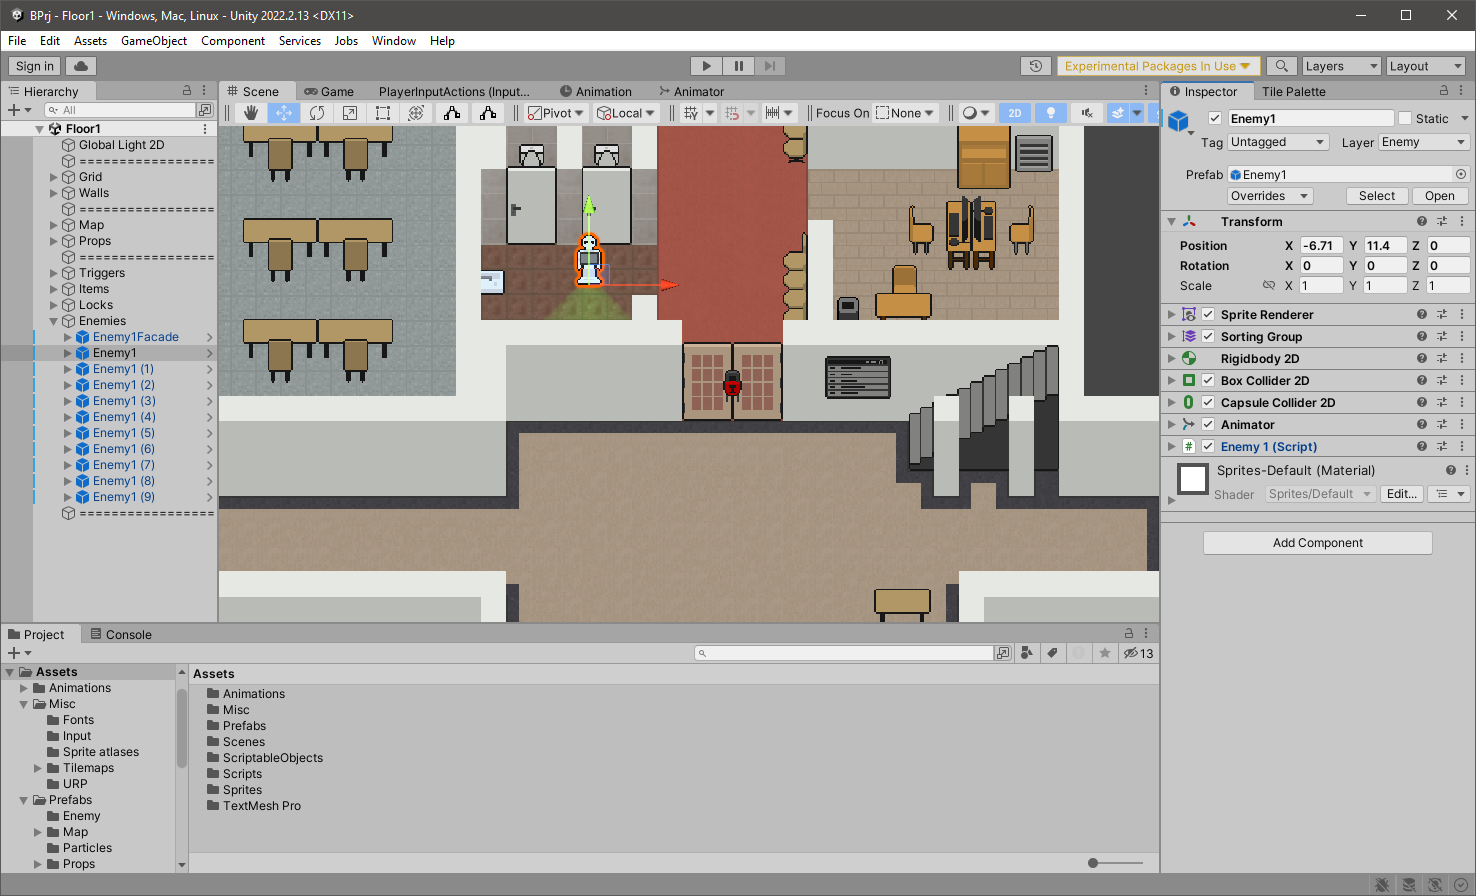
\includegraphics[width=\textwidth]{img/UnityEditor}
		\caption{Unity editor}
	\end{figure}
	
	\section{2D tvorba}
	
	Unity vzniklo původně jako engine pro vývoj 3D her a nástroje pro 2D tvorbu byly přidány až v pozdějších verzích. Volba mezi 2D a 3D je prvním krokem při zakládání nového projektu, rozdíl mezi nimi ale není velký a oba přístupy lze během vývoje kombinovat. Hlavním viditelným rozdílem pro 2D projekty je editor scény, který je přepnut do dvourozměrného režimu. V tomto módu je změněn význam osy Z, která místo popisu třetího rozměru značí hloubku (podobně jako např. vlastnost z-index v CSS). \cite{Unity2DAnnouncement}
	
	\subsection{Sprite} %spriteshape, atlas;
	
	Sprite je jeden z nejběžnějších assetů ve 2D videohře. V Unity vzniká přetažením bitmapového obrázku do průzkumníka projektu (obvykle do složky \textit{Sprites}) a má několik vlastností, které lze změnit v inspektoru. Za zmínku stojí hodnota \textit{Pixels Per Unit}, která určuje, kolik pixelů ve spritu odpovídá jednotce vzdálenosti v herním světě (ve scéně). Druhý důležitý parametr je \textit{Pivot}, ten značí bod, kolem kterého sprite rotuje, a také může ovlivnit pořadí vykreslení daného spritu.
	
	Každý sprite nemusí být reprezentován samostatným bitmapovým souborem, místo toho lze naimportovat tzv. spritesheet. Jedná se o větší obrázek obsahující více spritů uspořádaných do mřížky, ty jsou pak rozděleny na jednotlivé assety v nástroji editor spritů. Tento nástroj také umožňuje připravit obrázek pro specifický typ škálování zvaný 9-slicing (obrázek \ref{img9Slicing}).
	
	\begin{figure}[ht]
		\centering
		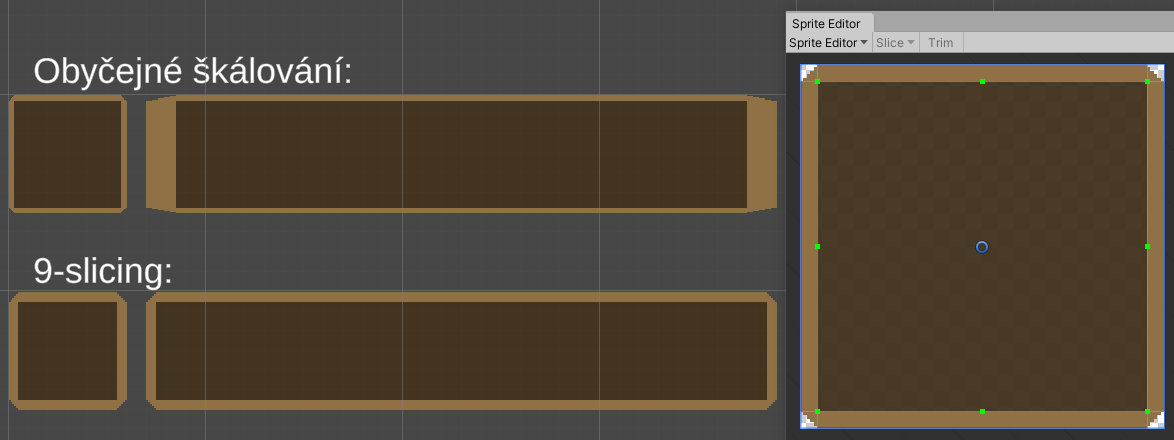
\includegraphics[width=\textwidth]{img/9Slicing}
		\caption{9-slicing}
		\label{img9Slicing}
	\end{figure}
	
	\subsection{Animace}
	
	Unity umožňuje tvorbu animací po jednotlivých snímcích, kdy je každý snímek animace reprezentován samostatným spritem. Jednotlivé sprity jsou pokládány na časovou osu v nástroji \textit{Animation}. Nevýhoda této metody se projeví v situaci, kdy je potřeba např. nějaké postavě změnit barvu vlasů. V tomto případě je nutné všechny sprity všech animací postavy upravit v (externím) grafickém editoru. Problém by šel také vyřešit tvorbou speciálního shaderu nebo editací jednotlivých pixelů ze skriptu, nejedná se ale o standardní postupy. Alternativně lze použít metodu trojúhelníkové sítě a kostry. Jedná se o běžný způsob tvorby 3D animací, Unity jej ale umožňuje aplikovat i na 2D sprity.
	
	Každý herní objekt schopný animace musí mít přiřazený asset typu \textit{Animator Controller} (dále jen AC). Ten je vytvořen a upravován přímo v Unity editoru a jeho diagram připomíná schéma stavového automatu. Všechny animace, ve kterých se herní objekt může nacházet, jsou v diagramu reprezentovány obdélníkem. Obdélníky lze spojovat šipkami, které značí podmíněný přechod mezi jednotlivými animacemi. AC umožňuje definovat si v něm interní proměnné (\textit{parameters}), jejichž hodnoty lze měnit ze skriptu a využívají se pro sestavení podmínek přechodu. AC diagramy složitějších herních objektů mohou značně nabýt na složitosti, je možné se jim ale vyhnout. Volání funkce \textit{Animator.CrossFade} dovoluje změnit animaci kdykoliv bez ohledu na stav AC diagramu.
	
	\subsection{Tilemap}
	
	Tilemap je nástroj pro tvorbu herních světů převážně ve 2D. Základem je pravidelná mřížka, do které jsou vkládány dlaždice (\textit{tiles}). Dlaždice je malý sprite nakreslený tak, aby více dlaždic položených vedle sebe vypadalo přirozeně a dala se z nich takto poskládat celá herní mapa. Využitím tilemap lze tvořit velké herní mapy bez dopadu na výkon a zároveň je kdykoliv snadno editovat. Unity nabízí obdélníkovou tilemap (nejběžnější, vhodné pro plošinovky a top-down videohry), ale také šestiúhelníkovou nebo izometrickou. V jedné scéně se může nacházet více tilemap a každá může být v jiné vrstvě. To např. umožňuje, aby se některé dlaždice vykreslovaly před a některé za postavou hráče.
	
	\textit{Rule Tile} je speciální druh dlaždice, která mění svůj vzhled na základě jednoduchých nastavitelných pravidel. Sprite této dlaždice se mění podle toho, zdali se v jejím okolí nachází dlaždice stejného druhu. Funkcionalita je ale omezená, nelze např. nastavit, aby dlaždice reagovala na své sousedy z jiných vrstev nebo na jiné dlaždice ve stejné vrstvě.
	
	\begin{figure}[ht]
		\centering
		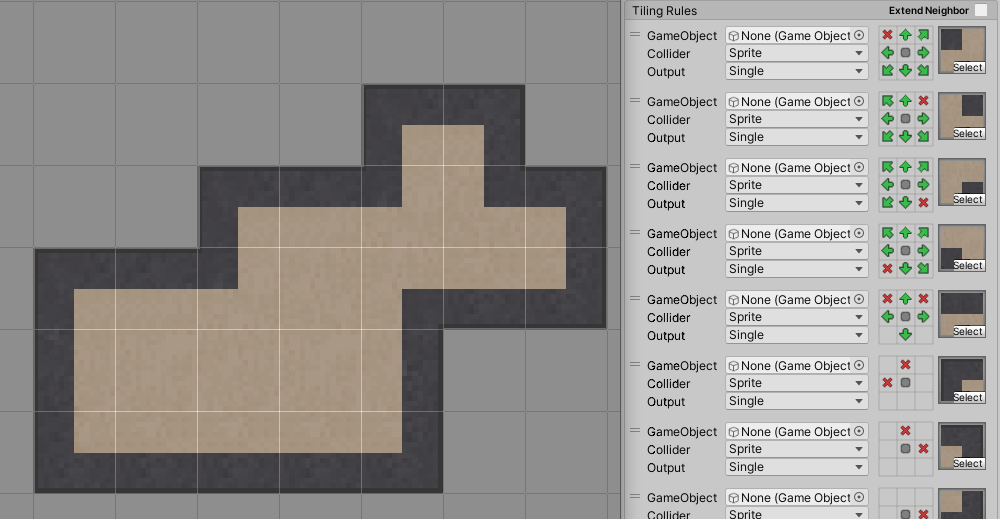
\includegraphics[width=\textwidth]{img/RuleTile}
		\caption{Rule Tile}
	\end{figure}
	
	\subsection{Universal Render Pipeline}

	Universal Render Pipeline (URP) je skriptovatelný vykreslovací řetězec, který je do Unity projektu přidán ve formě balíku. Otázka použití alternativního vykreslovacího řetězce bývá častější u vývoje 3D her, i pro 2D projekty ale URP přináší nové grafické možnosti. Tím nejzásadnějším jsou dvě nové komponenty \textit{Light 2D} a \textit{Shadow Caster 2D}, díky kterým lze do scény přidat dynamická světla a stíny.
	
	\chapter{Návrh videohry}
	% Vymyslete koncept a herní mechaniky pro 2D top-down videohru.	Rozmyslete si, jak bude hráč ovládat postavu, jaké budou cíle a výzvy ve hře a jakému prostředí a překážkám budou hráči čelit.	
	% * Základní přehled – premisa; perspektiva; žánr
	% * Žánr podrobněji, jednotlivé herní mechaniky (co všechno hráč může dělat ?)
	% * Zasazení podrobněji, level design
	% * Art style
	% * ..., technologické detaily, story, audio
	
	\section{Příběh} %přidat zasazení ?, úkoly
	
	Navrhovaná hra tohoto projektu uvádí hráče do role maturanta, který se chystá na FM podat přihlášku ke studiu. Po vstupu na fakultu se za ním zavřou a uzamknou dveře. Novým cílem je tedy zjistit, co se děje. Posléze je hráč kontaktován osobou, která ho informuje, že celou budovu fakulty má pod kontrolou místní umělá inteligence, jež se vymkla kontrole.
	
	Hlavním cílem hry je zastavit umělou inteligenci a uniknout z fakulty. V budově se nachází nepřátelští roboti, kteří se v tom hráči pokusí zabránit. Zhruba v druhé polovině příběhu se hráč dozvídá, že osoba, jež ho kontaktovala, byla ve skutečnosti samotná umělá inteligence, která ho tímto využívala. Koncept příběhu je inspirován herní sérií System Shock.
	
	\section{Žánr}
	
	Obecně by se hra dala kategorizovat jako akční a nabízí dva základní styly hraní. Tím prvním je boj na blízko. Hráč má k dispozici zbraň, konkrétně se jedná o hasák, se kterou může útočit na nepřátele. Ti mohou stejným způsobem zase útočit na hráče. Po každém úspěšném zásahu je cíli útoku ubráno jeho zdraví, které je v případě této hry reprezentováno celým číslem, a jakmile se dostane na nulu, tak je cíl zneškodněn.
	
	Druhou možností pro hráče je vyhnout se přímé konfrontaci s nepřáteli a namísto toho se před nimi skrývat. Žánr, kde se hráč snaží, aby nebyl odhalen nepřátelskými jednotkami, se ve videoherní terminologii nazývá stealth game. Slovem stealth se označuje i hlavní mechanika tohoto žánru – plížení, které hráči pomáhá nebýt spatřen.
	
	\section{Vizuální stránka}
	
	Hra je zobrazována pohledem kamery, která na mapu pohlíží svrchu. Tato perspektiva bývá obecně nazývána jako top-down. V případě tohoto projektu není kamera namířena přímo kolmo na plochu mapy, ale sleduje herní svět pod úhlem přibližně 45 stupňů. Pohled pod určitým úhlem odhaluje hloubku vyobrazovaných objektů a přesněji by se dal nazvat jako axonometrická projekce.
	\cite{MatejJan}
	
	Grafika hry je nakreslena ve stylu pixel art. Jedná se o druh digitálního grafického umění, kde každý pixel ve výsledném obraze hraje svou roli a změna jediného pixelu může značně ovlivnit, jak obraz na pozorovatele působí. Počátky pixel artu sahají do dob 8 a 16bitových konzolí, kde byla omezená paleta barev a rozlišení zobrazovaných spritů. Svou důležitost si ale pixel art zachoval dodnes. Je oblíbený zejména mezi nezávislými vývojáři kvůli jednoduchosti a rychlosti tvorby.
	\cite{pixelArt}
	
	V grafickém stylu této hry není dodrženo pravidlo užití omezené palety barev. Sprite postavy hráče má rozměry 16 na 32 pixelů a od toho jsou přibližně odvozeny velikosti všech ostatních spritů. Kromě dlaždic pro tilemap mají všechny sprity přidán tmavý obrys o šířce jednoho pixelu, aby vynikly a nesplývaly s pozadím.
	
	\begin{figure}[ht]
		\centering
		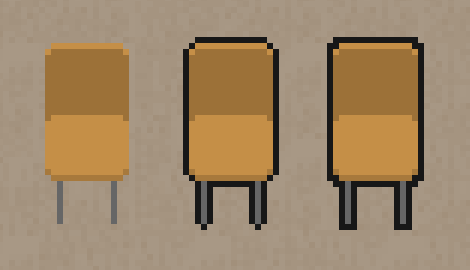
\includegraphics[width=0.5\textwidth]{img/SpriteBorder}
		\caption{Druhy obrysů u spritu}
	\end{figure}
	
	\section{Herní mechaniky}
	
	\subsection{Pohyb} % WASD, Dash, Stamina, Door Lock&Key, Ctrl, Airvents, stealth
	
	Postava hráče se může pohybovat v osmi směrech pomocí kláves W, A, S a D. Stiskem mezerníku se provede rychlý úskok (dash), během kterého je postava nezranitelná. Dash ubírá hráčovu staminu, která se časem regeneruje na svou původní hodnotu, a nelze ho provést, pokud není staminy dostatek.
	
	Aby hráč nenavštěvoval jednotlivé lokace na herní mapě v pořadí, které by porušilo konzistenci příběhu, je jeho pohyb omezen pomocí uzamčených dveří. Aby tyto dveře mohly být otevřeny, musí nejprve hráč nalézt klíč v barvě odpovídající zámku na daných dveřích.
	
	Stiskem klávesy Ctrl se postava hráče skrčí a přepne do režimu plížení. V tomto módu se pohybuje pomaleji, ale může pro přesun využít větracích šachet rozmístěných po mapě. Hráč ve větrací šachtě nemůže být spatřen nepřítelem. To samé platí, pokud je v režimu plížení schovaný za nějakým objektem (např. za stolem).
	
	\subsection{Boj} % attack, cooldown, dead + RESPAWN
	
	Stiskem levého tlačítka myši (LMB) se provede útok na blízko, ten si bere malou část staminy a na chvíli pozastavuje její regeneraci. Útok má také svou vlastní dobíjecí dobu, aby nemohl být opakován jeden za druhým bez jakékoliv pauzy (attack spamming). Po vypršení dobíjecí doby následuje krátké časové okénko, během kterého stisknutí LMB provede útok s kritickým zásahem, který ubírá více bodů zdraví. Pokud naopak hráč stiskne LMB během dobíjecí doby, již není možné provést útok s kritickým zásahem a dobíjecí doba se o toto časové okénko prodlouží.
	
	Hráč má svou hladinu zdraví, která se, pokud nebyl po určitou dobu zraněn nepřítelem, regeneruje do poloviny své maximální kapacity. Pokud hráčovo zdraví klesne na nulu, neznamená to konec hry. Namísto toho je hráč oživen (respawn) ve vestibulu budovy s tím, že jeho aktuální úkol, sebrané předměty a zneškodnění nepřátelé nejsou resetováni.
		
	\subsection{Grafické uživatelské rozhraní} % Tutorial, inspect&interact, pauza, dialogue
	
	Pro informování hráče ohledně hodnot určitých atributů se používá heads-up display (HUD). Jedná se o samostatnou vrstvu, která je vykreslena nad herním světem a její pozice na obrazovce je fixní. V pravé dolní části obrazovky je napsána informace o právě zkoumaném objektu ve hře. Jedná se o objekt, na který uživatel najede kurzorem. Na prvním řádku je zobrazen název tohoto objektu a pokud s ním lze nějakým způsobem interagovat, tak je na druhém řádku napsán název příslušné akce (např. otevření dveří). Při zkoumání nepřátelské jednotky je na druhém řádku vykreslena hladina jejího zdraví. Ukazatele hráčova zdraví a staminy se nachází v levé dolní části obrazovky.
	
	Pokud je pro hráče k dispozici nový tutoriál, tak se nad těmito dvěma ukazateli zobrazí oznámení. Stiskem klávesy tabulátoru se otevře okno s tutoriálem. Jedná se o stručnou nápovědu popisující, jak se má hra ovládat a jak fungují základní mechaniky. Na začátku hry je k dispozici pouze první tutoriál popisující pohyb postavy a další nápověda se zpřístupní ve chvíli, kdy je relevantní.
	
	\section{Umělá inteligence}	
	% Vytvořte jednoduchý systém umělé inteligence pro nepřátelské jednotky ve hře, který bude řízen stavovým automatem. Uvažujte o různých stavech, ve kterých se může nepřítel nacházet (např. hlídka, útok, ústup), a jak tyto stavy ovlivní chování nepřátelských jednotek.
	% * FSM obecně
	% * Enemy FSM
	% * A*
	% * Implementace ?
	
	Hra obsahuje nepřátelskou jednotku s jednoduchou umělou inteligencí řízenou konečným stavovým automatem. Výchozí činností nepřítele je hlídkovat libovolný počet bodů na mapě. Jakmile nepřítel zahlédne postavu hráče, vydá se toto místo prozkoumat a popřípadě na hráče zaútočí. Nepřítel využívá algoritmu A*, aby věděl, jakou cestou se vydat ke svému aktuálnímu cíli.
	
	Je třeba zmínit, že pojem \quotedblbase umělá inteligence\textquotedblleft\ v kontextu videoherní tvorby obvykle neznamená algoritmus řešící komplexní problémy na základě datové analýzy. Cílem je vytvořit chování nehráčských postav, které zlepšuje herní zážitek. Předvídatelnost a čitelnost může mít při návrhu takového algoritmu prioritu před simulací reálného lidského chování.
	\cite{gameAI}
	
	\subsection{Konečný stavový automat}
	
	Konečný stavový automat (finite state machine, FSM) je výpočetní model běžně používaný ve videohrách pro implementaci umělé inteligence nehráčských postav. Objekt implementující FSM má definovaný konečný počet stavů a vždy se musí nacházet právě v jednom z nich. V případě her jednotlivé stavy reprezentují akce a činnosti, které mohou nehráčské postavy vykonávat. K návrhu FSM lze použít graf, kde je pro každý stav vytvořen příslušný vrchol a orientované hrany mezi těmito vrcholy značí podmíněné přechody mezi stavy. Objekt se tedy přepne z jednoho stavu do jiného, pokud mezi těmito stavy existuje přechod a jsou splněny jeho podmínky.
	\cite{lit1}
	
	\subsection{Nepřátelská jednotka – návrh}
	
	Výchozím stavem nepřátel v této hře je stav hlídky \textit{PatrolState}. Nepřítel hlídkuje mezi jednotlivými body na mapě, které má v sobě uložené jako kolekci dvourozměrných souřadnic. Jakmile se dostane na souřadnice stanoviště, zastaví se a přepne do stavu rozhlížení \textit{LookAroundState}, po kterém následuje opět stav hlídky. Tentokrát má ale tento stav jako stanoviště nastavené následující souřadnice z kolekce. Mezi těmito dvěma stavy takto nepřítel přepíná do té doby, než se do jeho zorného pole dostane postava hráče.
	
	Zorné pole nepřátel je ve hře vizualizováno pomocí barevné kruhové výseče, která je vykreslena na zemi tak, že střed kružnice leží nepříteli u nohou a její poloměr je roven délce dohledu nepřítele. Tvar této výseče se dynamicky mění, aby odpovídal tomu, kde nepřítel může a nemůže spatřit hráče. Pokud se tedy např. hráč krčí za stolem, tak je zkrácena délka paprsků výseče, které se stolem kolidují.
	
	Výchozí barvou výseče během stavu hlídky je zelená. Jakmile do zorného pole nepřítele vstoupí hráč, změní výseč svou barvu na žlutou a nepřítel se přepne do stavu detekce \textit{DetectingState}. Pokud se hráč v určitém čase nestihne skrýt, pak nepřítel přejde do stavu pronásledování \textit{ChaseState}. Tento čas, během kterého má hráč šanci se ukrýt a nebýt detekován, je také vizualizován. Nad žlutou výsečí je vykreslena druhá červená výseč stejného tvaru, jejíž poloměr se postupně zvětšuje a jakmile se její okraj dostane až k hráči, znamená to, že byl detekován. Během stavu hlídky se pak poloměr červené výseče zmenšuje zpět na nulu. Tento druh zobrazení zorného pole a hladiny podezření nepřátelských jednotek je inspirován hrou Shadow Tactics: Blades of the Shogun.
	
	Při stavu pronásledování nepřítel stíhá hráče a když se dostane dostatečně blízko, tak na něj zaútočí (\textit{AttackState}). Pokud hráč zmizí z jeho dohledu, přechází nepřítel do stavu průzkumu \textit{InvestigateAwareState}, kde je cílem jeho cesty poslední pozice, na které byl hráč viděn. Spatření hráče během tohoto stavu znamená opětovné pronásledování, jinak, jakmile se dostane na konec své cesty, se nepřítel vrátí k rutině neutrálních stavů hlídka a rozhlížení. Podobně funguje stav \textit{InvestigateSuspiciousState} s tím rozdílem, že do něj se lze dostat ze stavu detekce a spatření hráče tedy znamená opětovnou detekci.
	
	Posledním stavem je \textit{KnockbackState} (vynechán z obrázku \ref{imgFSM} kvůli přehlednosti). Do něj se nepřítel dostane po obdržení zásahu od hráče. V tomto stavu je mírně odstrčen ve směru obdrženého útoku a následně se vrací do stavu útoku, pronásledování, nebo průzkumu podle toho, jak daleko se od něj nachází hráč a zdali je vůbec v jeho zorném poli.
	
	\begin{figure}[ht]
		\centering
		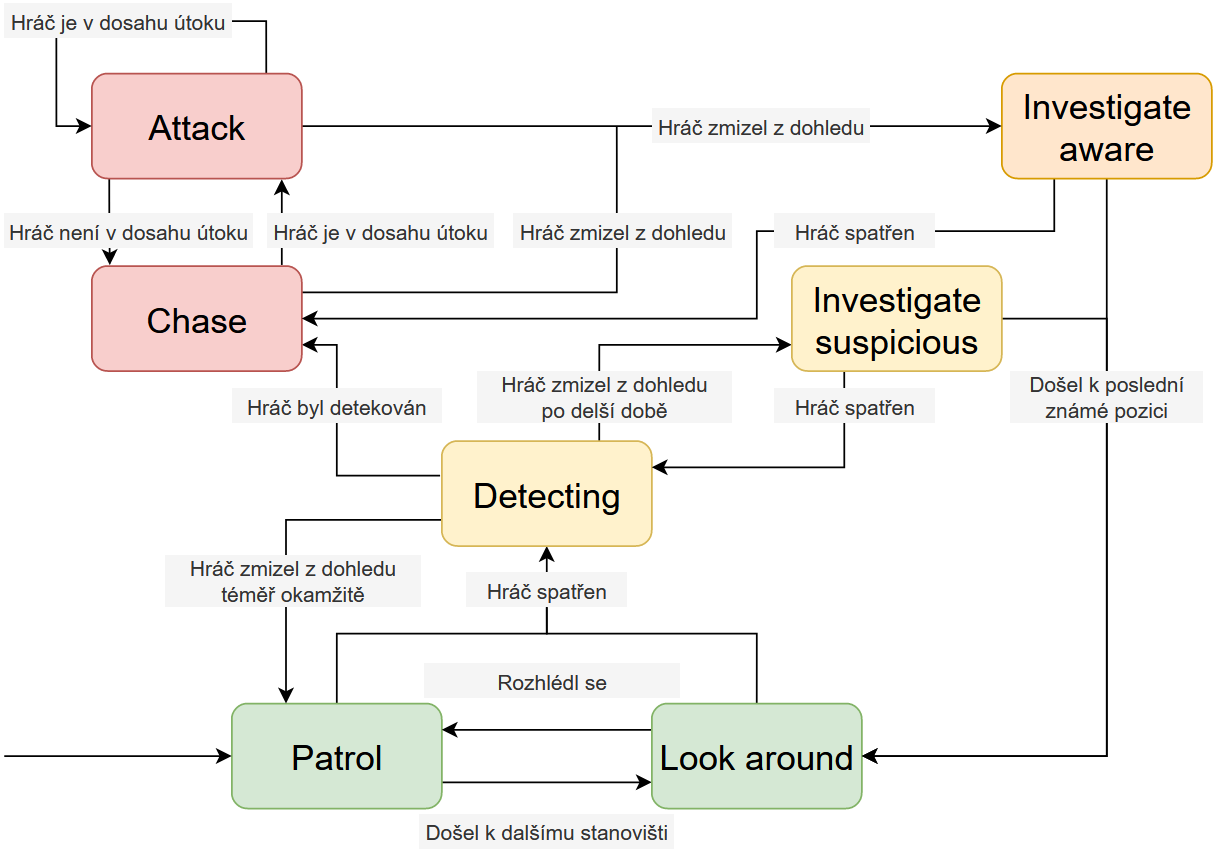
\includegraphics[width=\textwidth]{img/FSM}
		\caption{Graf stavového automatu nepřátelské jednotky}
		\label{imgFSM}
	\end{figure}
	
	% A* a případ: patrol -> investigateAware řešit až v implementaci ?
	
	\chapter{Implementace}
	% Implementace demonstrativní videohry v prostředí budovy FM TUL.
	% * Unity
	% * Grafika, animace
	% * Player State Machine
	% * Tilemap a tvorba mapy; sprite atlas; cinemachine
	% * YSorting problémy
	% * HUD – observer, inspect, dialogue; tutorial
	% * Enemy, pathfinding, view cone, player vision/detection/chase/...
	% * Triggers, consistency manager, managers, menu, ...
	
	Po návrhu videohry následovala její implementace, která začala založením prázdného 2D projektu v Unity 2021. Byla zvolena verze 2021, protože se jedná o verzi s dlouhodobou podporou a samo Unity ji v tuto chvíli doporučuje.
	
	Poté už se mohly začít tvořit jednotlivé assety. Prvním cílem bylo vytvořit postavu hráče a umožnit jí základní pohyb. To si vyžadovalo nakreslit sprity a z nich sestavit animace, napsat skripty pohybující s postavou hráče, ale také zprovoznit tilemap a pro základní testovací mapu.
	
	Implementace takto probíhala postupným nabalováním jednotlivých herních mechanik. Vždy se pracovalo na jedné konkrétní funkční části a dokud nebyla dotažena do uspokojivého stavu, nevěnoval se vývoj ničemu jinému. Tento postup vývoje byl validní, dokud se nedostal k tvorbě nepřátelské jednotky, která byla časově náročnější. Hra sice obsahovala nepřátelskou jednotku, která se postupně zlepšovala, ale čas určený pro praktickou část této práce se krátil a hra postrádala jakýkoliv příběh či mapu, na které by se příběh odehrával.
	
	Proto byl zvolen přístup tvorby minimálního životaschopného produktu. Prioritou bylo zhotovit hru, kterou lze dohrát od začátku do konce, a až poté se věnovat případným detailům, chybám a nedostatkům. Vývoj se po této změně zaměřoval převážně na herní mapu, příběh a grafické uživatelské rozhraní. Hra byla po dokončení své první verze odeslána malé skupince testerů, na základě jejichž zpětné vazby byly doladěny některé herní mechaniky a opraveny nalezené chyby.
	
	\section{Grafika} % GIMP, animace
	
	Unity v sobě nemá zabudovaný žádný grafický editor, pro tvorbu spritů do 2D hry je ale možné použít jakýkoliv program s podporou průhlednosti. Vhodným nástrojem pro tvorbu herní grafiky ve stylu pixel art je program Aseprite, pro tento projekt byl ale zvolen  GIMP kvůli své bezplatné licenci a předchozím zkušenostem s tímto programem.
	
	V programu GIMP byla většina potřeb grafiky této hry pokryta nástrojem tužka. Vhod přišla také možnost nechat si v obrázku vykreslit mřížku oddělující jednotlivé snímky ve spritesheetu. GIMP nemá žádné podpůrné nástroje pro tvorbu animací. Ty proto vznikaly tak, že byly nakresleny jejich jednotlivé snímky, v Unity se z nich vytvořila animace a teprve v té chvíli si bylo možné animaci prohlédnout. Kvůli neintuitivnosti a časové náročnosti tohoto procesu se nakonec postava hráče stala jediným objektem ve hře, který disponuje animacemi složenými z více snímků.
	
	\begin{figure}[ht]
		\centering
		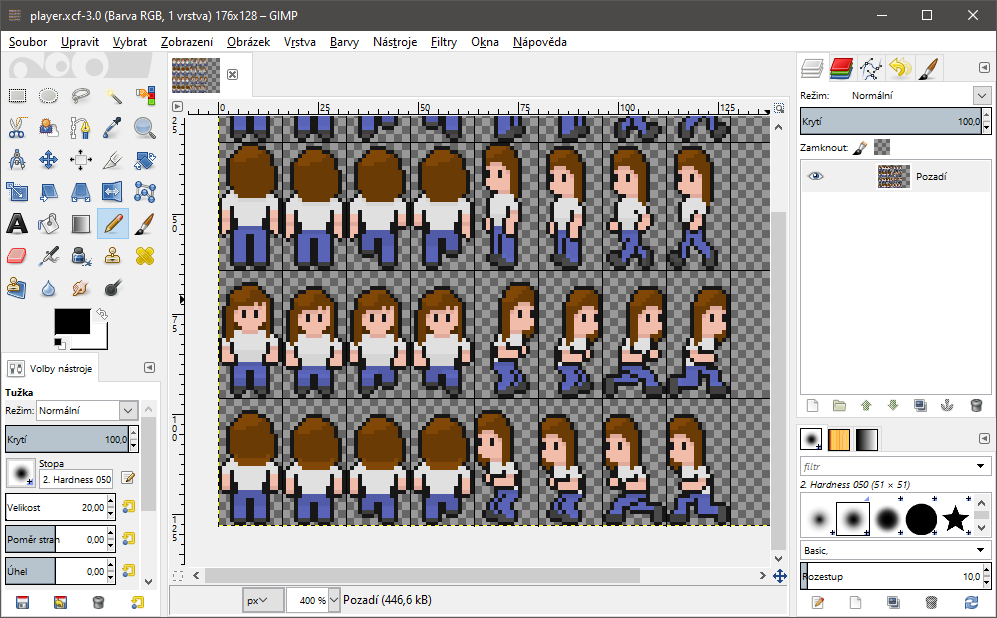
\includegraphics[width=\textwidth]{img/GIMP}
		\caption{Program GIMP}		
	\end{figure}
	
	\section{Postava hráče} % FSM stavy – idle, move, sneak, attack, dash, (dialogue, dead, knockback)
	
	Postava hráče využívá stejnou implementaci stavového automatu jako jednotka nepřítele (podrobněji popsáno v sekci \ref{chpFSM}). FSM je typičtější používat pro nehráčské postavy, i zde se dá ale využít jeho výhod. Kód je logicky členěn do souborů podle jednotlivých činností, které může hráč vykonávat. Přechody mezi jednotlivými stavy jsou v tomto případě většinou podmíněny stiskem nějaké klávesy.
	
	\textit{Rigidbody2D}.
	
	\section{Herní mapa} % Tilemap, problémy s perspektivou
	
	\section{Nepřátelská jednotka – implementace} % FSM, URP, A*
	\label{chpFSM}
	
	\section{Příběh a postup hrou}
	 
	\chapter{Kritické zhodnocení}
	% Výslednou videohru kriticky zhodnoťte a navrhněte případné rozšíření či vylepšení.
	
	\chapter{Závěr}
	
	% Zdroje
	\chapter*{Seznam použité literatury}
	\addcontentsline{toc}{chapter}{Seznam použité literatury}
	\printbibliography[heading=none]
	
\end{document}